% Options for packages loaded elsewhere
\PassOptionsToPackage{unicode}{hyperref}
\PassOptionsToPackage{hyphens}{url}
\PassOptionsToPackage{dvipsnames,svgnames*,x11names*}{xcolor}
%
\documentclass[
]{article}
\usepackage{lmodern}
\usepackage{amssymb,amsmath}
\usepackage{ifxetex,ifluatex}
\ifnum 0\ifxetex 1\fi\ifluatex 1\fi=0 % if pdftex
  \usepackage[T1]{fontenc}
  \usepackage[utf8]{inputenc}
  \usepackage{textcomp} % provide euro and other symbols
\else % if luatex or xetex
  \usepackage{unicode-math}
  \defaultfontfeatures{Scale=MatchLowercase}
  \defaultfontfeatures[\rmfamily]{Ligatures=TeX,Scale=1}
\fi
% Use upquote if available, for straight quotes in verbatim environments
\IfFileExists{upquote.sty}{\usepackage{upquote}}{}
\IfFileExists{microtype.sty}{% use microtype if available
  \usepackage[]{microtype}
  \UseMicrotypeSet[protrusion]{basicmath} % disable protrusion for tt fonts
}{}
\makeatletter
\@ifundefined{KOMAClassName}{% if non-KOMA class
  \IfFileExists{parskip.sty}{%
    \usepackage{parskip}
  }{% else
    \setlength{\parindent}{0pt}
    \setlength{\parskip}{6pt plus 2pt minus 1pt}}
}{% if KOMA class
  \KOMAoptions{parskip=half}}
\makeatother
\usepackage{xcolor}
\IfFileExists{xurl.sty}{\usepackage{xurl}}{} % add URL line breaks if available
\IfFileExists{bookmark.sty}{\usepackage{bookmark}}{\usepackage{hyperref}}
\hypersetup{
  colorlinks=true,
  linkcolor=red,
  filecolor=Maroon,
  citecolor=Blue,
  urlcolor=Blue,
  pdfcreator={LaTeX via pandoc}}
\urlstyle{same} % disable monospaced font for URLs
\usepackage[margin=1in]{geometry}
\usepackage{graphicx}
\makeatletter
\def\maxwidth{\ifdim\Gin@nat@width>\linewidth\linewidth\else\Gin@nat@width\fi}
\def\maxheight{\ifdim\Gin@nat@height>\textheight\textheight\else\Gin@nat@height\fi}
\makeatother
% Scale images if necessary, so that they will not overflow the page
% margins by default, and it is still possible to overwrite the defaults
% using explicit options in \includegraphics[width, height, ...]{}
\setkeys{Gin}{width=\maxwidth,height=\maxheight,keepaspectratio}
% Set default figure placement to htbp
\makeatletter
\def\fps@figure{htbp}
\makeatother
\setlength{\emergencystretch}{3em} % prevent overfull lines
\providecommand{\tightlist}{%
  \setlength{\itemsep}{0pt}\setlength{\parskip}{0pt}}
\setcounter{secnumdepth}{-\maxdimen} % remove section numbering
\usepackage{pdfpages}
\usepackage{amsmath}
\usepackage{placeins}
\usepackage{booktabs}
\usepackage{longtable}
\usepackage{array}
\usepackage{multirow}
\usepackage{wrapfig}
\usepackage{float}
\usepackage{colortbl}
\usepackage{pdflscape}
\usepackage{tabu}
\usepackage{threeparttable}
\usepackage{threeparttablex}
\usepackage[normalem]{ulem}
\usepackage{makecell}
\usepackage{xcolor}
\newlength{\cslhangindent}
\setlength{\cslhangindent}{1.5em}
\newenvironment{cslreferences}%
  {}%
  {\par}

\author{}
\date{\vspace{-2.5em}}

\begin{document}

\pagenumbering{gobble}

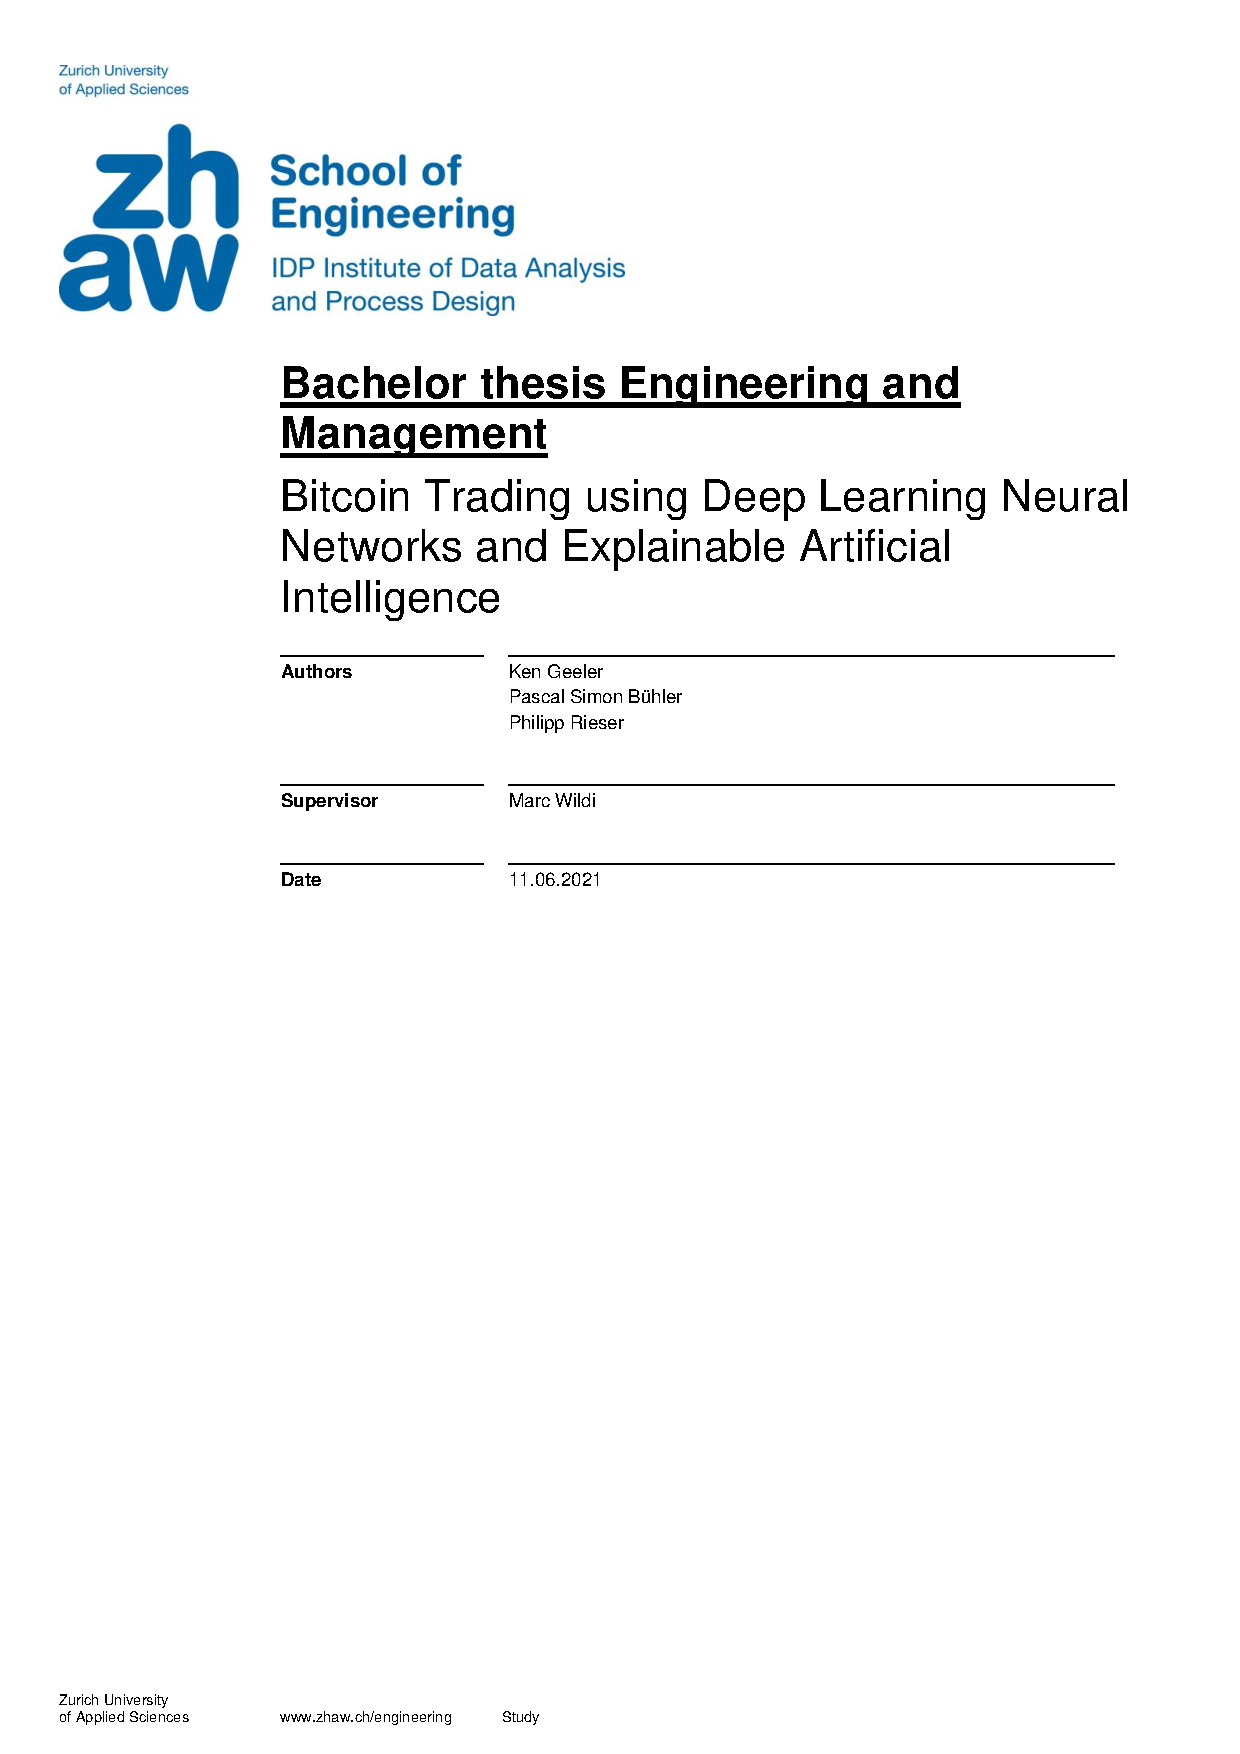
\includepdf{add/titlepage.pdf}

\includepdf{add/declaration.pdf}

\setcounter{tocdepth}{4}
\tableofcontents

\newpage

\hypertarget{abstract}{%
\subsection{Abstract}\label{abstract}}

\newpage

\pagenumbering{arabic}

\hypertarget{introduction}{%
\subsection{1. Introduction}\label{introduction}}

Ken is testing working with Github.does it work now?

\hypertarget{intro}{%
\subsubsection{1.1. Intro}\label{intro}}

\newpage

\hypertarget{theory}{%
\subsection{2. Theory}\label{theory}}

The following chapter is intended to provide the theoretical foundations
necessary for our work. It is divided into a part that provides an
overview of artificial neural networks. Followed by section
\protect\hyperlink{bitcoin}{2.2.} which shows the background and the
ecosystem of Bitcoin. This knowledge should be kept in mind, which
should help in understanding the price formation of Bitcoin.

\hypertarget{neural_network}{%
\subsubsection{2.1. Neural network}\label{neural_network}}

In the context of this work, artificial neural networks are used to
answer supervised learning questions that focus on the classification of
data. This means that a neural network finds a correlation between the
data and their labels and optimizes its parameters to minimize the error
for the next try. This process is called supervised training and is
performed with a test data sample. An application example of
classification is that a neural network is used for face recognition
after it has learned the classification of different faces in the
process of supervised training. Predictive analysis works similarly to
the classification of labeled data. It estimates future values based on
past events and can be trained with historical data. On the other hand,
unsupervised learning (clustering) is applied to detect patterns from
unlabeled data. Based on these patterns, for example, anomalies can be
detected that are relevant in the fight against fraud (fraud detection).
Unsupervised learning is not discussed further in this paper. Section
\protect\hyperlink{perceptron}{2.1.1.} will demonstrate the functioning
of a neural network using a simple perceptron.

\hypertarget{perceptron}{%
\paragraph{2.1.1. Perceptron}\label{perceptron}}

~

The construction of an artificial neural network is demonstrated using a
perceptron. It is a simple algorithm for supervised learning of binary
classification problems. This algorithm classifies patterns by
performing a linear separation. Although this discovery was anticipated
with great expectations in 1958, it became increasingly apparent that
these binary classifiers are only applicable to linearly separable data
inputs. This was only later addressed by the discovery of multiple layer
perceptrons (MLP) {[}1{]}. Basically, a perceptron is a single-layer
neural network and consists of the following five components and can
also be observed in figure \ref{fig:perceptron_schema}.

\begin{enumerate}
\def\labelenumi{\arabic{enumi}.}
\item
  Inputs
\item
  Weights
\item
  Bias
\item
  Weighted sum
\item
  Activation function
\end{enumerate}

Inputs are the information that is fed into the model. In the case of
econometric time series, it is mostly the current and historical log
returns (lags). These are multiplied by the weights and added together
with the bias term to form the weighted sum. This weighted sum is
finally passed on to the non-linear activation function, which
determines the output of the perceptron.

\newpage

\begin{figure}

{\centering 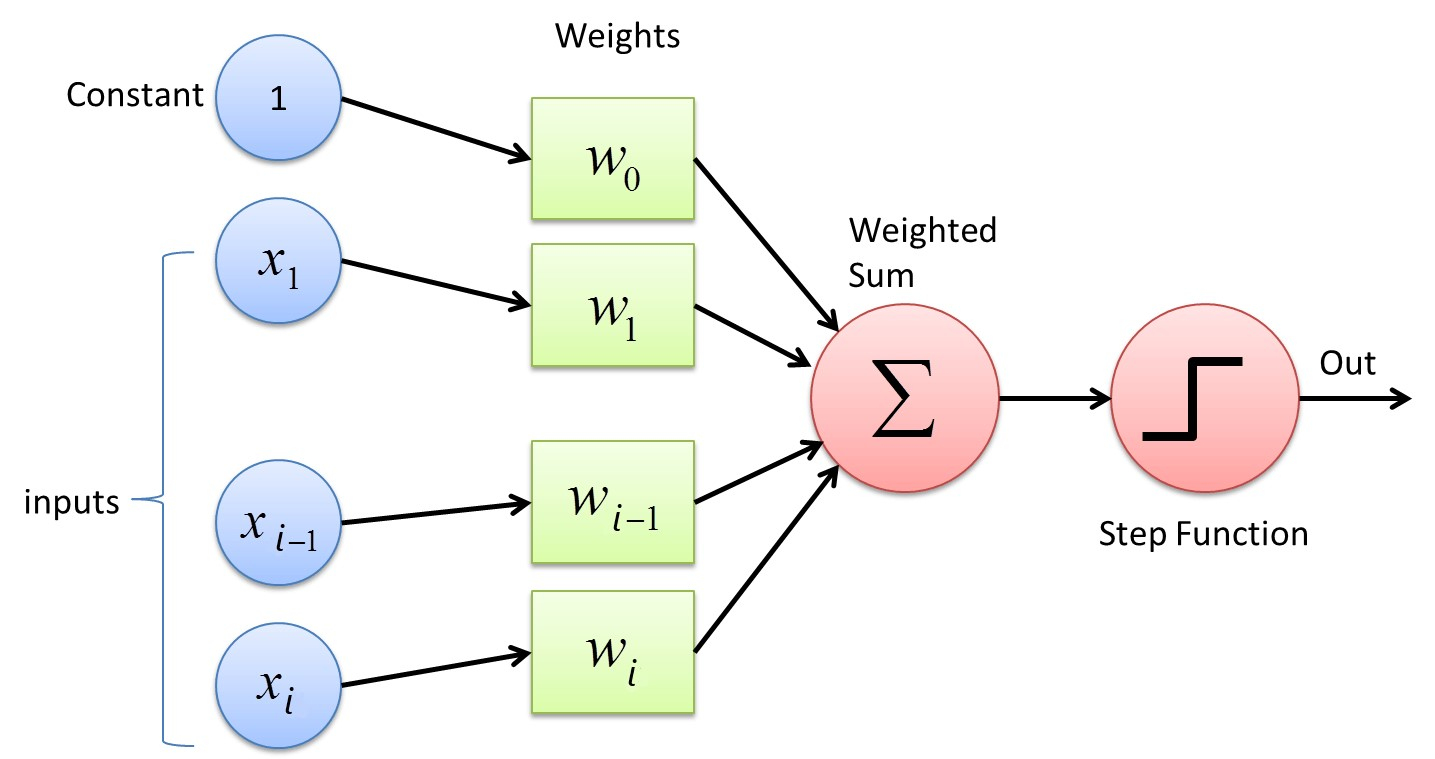
\includegraphics[width=0.7\linewidth]{images/Perceptron} 

}

\caption{Schematic diagram of a perceptron.}\label{fig:perceptron_schema}
\end{figure}

The perceptron can also be represented as a function, which can be seen
in equation \ref{eq:perceptron}. Analogous to the representation above,
the inputs \(x_{i}\) are multiplied by the weights \(w_{i}\) in a linear
combination. Then an error term is added so that the whole can be packed
into the non-linear activation function \(g(S)\) . \(\hat{y}\) is the
binary output of this perceptron. With the aid of an activation
function, binary output is obtained. The Heaviside step function shown
in figure \ref{fig:perceptron_schema} is usually only used in single
layer perceptrons, which recognize linear separable patterns. For the
multi-layer neural networks presented later, step functions are not an
option, because in the course of the backpropagation algorithm the
gradient descent has to be minimized. This requires derivatives of the
activation function, which in the case of this Heaviside step function
equals 0. Because the foundation for the optimization process is
missing, functions like the sigmoid function or the hyperbolic tangent
function are used {[}2{]}. More about this topic is discussed in chapter
\protect\hyperlink{backprogation_algorithm}{2.1.2}.

\begin{align} \label{eq:perceptron}
\hat{y}=g(w_{0}+\sum_{i=1}^{n}x_{i}w_{i})
\end{align}

As just mentioned, the aim is to feed the perceptron with the training
set and change the weights \(w_{i}\) with each cycle so that the
prediction becomes more accurate. The output value is compared to the
desired value. Finally, the sign of the difference \(y-\hat{y}\)
determines whether the inputs of that iteration are added to or
subtracted from the weights. Ideally, the weights will gradually
converge and provide us with a usable model {[}2{]}.

\newpage

\hypertarget{backprogation_algorithm}{%
\paragraph{2.1.2. Backpropagation
algorithm}\label{backprogation_algorithm}}

~

Finding the optimal weights of the neural network is achieved by finding
the minimum of an error function. One of the most common methods for
this is the backpropagation algorithm. This algorithm searches for the
minimum of the error function by making use of a method called gradient
descent. The gradient method is used in numerics to solve general
optimization problems. In doing so, we progress (using the example of a
minimization problem) from a starting point along a descent direction
until no further numerical improvement is achieved. Since this method
requires the computation of the gradient of the error function after
each step, continuity and differentiability of this function must
necessarily be given. The step function mentioned above in section
\protect\hyperlink{perceptron}{2.1.1.} is therefore out of the question,
but a non-linear function such as the logistic and the hyperbolic
tangent functions (sigmoid) {[}3{]}. Both activation functions are
visible in figure \ref{fig:sigmoid}. While the target range of the
`ordinary' sigmoid function (equation \ref{eq:sigmoid_logistic}) is
between 0 and 1, the \(\hat{y}\) of the hyperbolic tangent function
(equation \ref{eq:sigmoid_tanh}) ranges between -1 and 1. \(v_{i}\)
equals the weighted sum including bias term.

\begin{eqnarray}
\hat{y}(v_{i})=(1+e^{-v_{i}})^{-1} \label{eq:sigmoid_logistic} \\
\hat{y}(v_{i})=\tanh(v_{i}) \label{eq:sigmoid_tanh}
\end{eqnarray}

\begin{figure}

{\centering 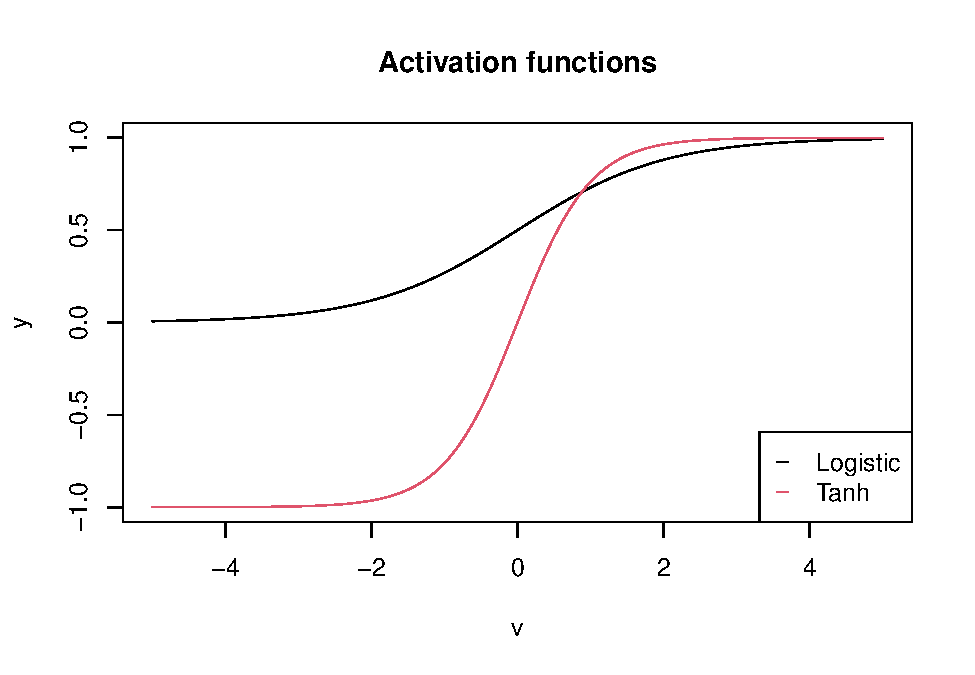
\includegraphics[width=0.7\linewidth]{00_main_files/figure-latex/sigmoid-1} 

}

\caption{Two common sigmoid activation functions: logistic functions and hyperbolic tangent.}\label{fig:sigmoid}
\end{figure}

In the course of the error analysis, the output of the neural network
respectively the result from the activation function in the output layer
is compared with the desired value. The most commonly used error
function E is the Mean Squared Error (MSE), which is seen in equation
\ref{eq:mse}. \(y_{i}\) represents the actual value for the data point
\(i\), while \(\hat{y}_{i}\) is the predicted value for data point
\(i\). The average of this error function is the average MSE, which is
determined for a corresponding model. The learning problem is to adjust
the weights \(w_{i}\) within the training sample so that \(MSE(w)\) is
minimized {[}4{]}.

\begin{align} \label{eq:mse}
  E &=MSE(w) \\
  &=\frac{1}{n}\sum_{i = 1}^{n}(y_{i}-\hat{y}_{i})^2 \nonumber \\
  &=\frac{1}{n}\sum_{i = 1}^{n}(y_{i}-g(w_{0}+x_{i}w_{i}))^2 \nonumber 
\end{align}

As mentioned, this is searched for by the gradient descent method. The
gradient of a function is a vector whose entries are the first partial
derivatives of the function. The first entry is the partial derivative
after the first variable, the second entry is the partial derivative
after the second variable and so on. Each entry indicates the slope of
the function in the direction of the variable to which it was derived.
In this work, the notation \(\nabla{E}\) is used when talking about the
gradient for the error function \(E\), which is displayed in equation
\ref{eq:gradient_descent} {[}3{]}.

\begin{align} \label{eq:gradient_descent}
\nabla{E}=(\frac{\partial E}{\partial w_{1}},
\frac{\partial E}{\partial w_{2}},
\dots,
\frac{\partial E}{\partial w_{i}})
\end{align}

The weights get adjusted according to the following algorithm
\ref{eq:weight_adj} where \(\Delta{w_{i}}\) is the change of the weight
\(w_{i}\) and \(\gamma\) represents a freely definable parameter. In
literature, this parameter is often called a learning constant {[}5{]}.
The negative value is used because the gradient naturally points in the
direction with the largest increase of the error function. To minimize
the MSE, the elements in the gradient \(\nabla{E}\) must be multiplied
by -1.

\begin{align} \label{eq:weight_adj}
\Delta{w_{i}}=-\gamma\frac{\partial E}{\partial w_{i}}, \\
\text{for } i=1,2,\dots,n \nonumber
\end{align}

\newpage

\hypertarget{MLP}{%
\paragraph{2.1.3. Multilayer perceptron}\label{MLP}}

~

Multilayer perceptrons (MLP) are widely used feedforward neural network
models and make usage of the backpropagation algorithm. They are an
evolution of the original perceptron proposed by Rosenblatt in 1958
{[}1{]}. The distinction is that they have at least one hidden layer
between input and output layer, which means that an MLP has more neurons
whose weights must be optimized. Consequently, this requires more
computing power, but more complex classification problems can be handled
{[}6{]}. Figure \ref{fig:mlp_schema} shows the structure of an MLP with
\(n\) hidden layers. Compared to the perceptron, it can be seen that
this neural network consists of an input layer, one or more hidden
layers, and an output layer. In each layer, there is a different number
of neurons, respectively nodes. These properties (number of layers and
nodes) can be summarized with the term `network architecture' and will
be dealt with in this thesis.

\begin{figure}

{\centering 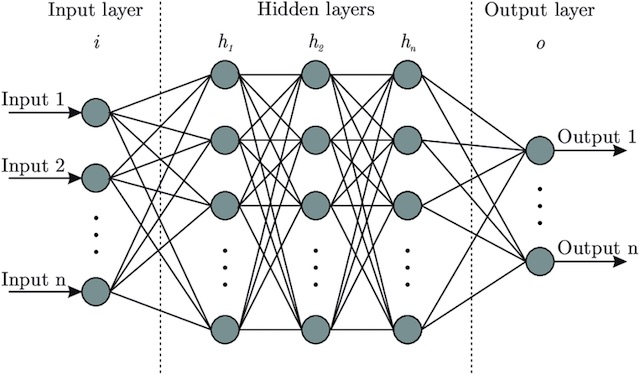
\includegraphics[width=0.6\linewidth]{images/MLP} 

}

\caption{Schematic diagram of a multilayer perceptron}\label{fig:mlp_schema}
\end{figure}

Every neural network has an input layer, which consists of one or more
nodes. This number is determined from the training data and tells us how
many features should be delivered to the neural network. In the case of
bitcoin prices, we could use today's price and the prices of the last 10
days (lags 1-10), so the input layer would consist of 11 nodes. Some
configurations also require a bias term to adjust the output along with
the weighted sum, which is also added to the input layer. In contrast to
the scheme of the MLP, this setup can be seen in figure
\ref{fig:perceptron_schema} where the bias term is defined as
`constant'. Similarly to the input layer, each neural network has
exactly one output layer. This can consist of one or more nodes. In this
thesis, MLP is used as a regressor and therefore only one neuron is
needed in this layer.

In between are the hidden layers, whose number and size can be
configured as desired. The challenge is to find an optimal and efficient
configuration without causing overfitting of the training data. The
number of hidden layers depends primarily on the application area of the
neural network. For example, working with image recognition would
require more layers since the image file is broken down into individual
pixels. Subsequently, the layers are used to optimize from rough
outlines to the smallest detail. In our research, we came across several
methods or `rules of thumb' to optimize the model. A frequently
suggested method is explained by Andrej Karpathy (director of the AI
department of Tesla, Inc.). His GitHub entry recommends the approach of
starting with a model that is too large that causes overfitting.
Subsequently, the model is reduced by focusing on increasing training
loss and improving validation loss {[}7{]}.

\hypertarget{RNN}{%
\paragraph{2.1.4. Recurrent neural networks (RNN)}\label{RNN}}

~

Recurrent neural networks (RNN) are a further development of
conventional neural networks. While MLP use new inputs \(x_i\) in each
epoch, RNN also use sequential data \(h_i\) in addition to \(x_i\). This
sequential data are called hidden states and result from the previous
runs. This has the advantage that historical information stemming from
past predictions is included for the prediction for \(t+1\). This effect
can be intuitively explained by an example in which the flight path of a
scheduled flight is predicted using RNN. When predicting the exact
location (coordinates) of a plane, it is of great advantage to know the
location at \(t-1\) and to derive the flight direction from it. With the
inclusion of this information, the target area can be narrowed down,
which optimally leads to more accurate results. The same principle is
used in applications like machine translation and speech recognition,
where the result (here possibly letter or word) of the last epoch plays
a big role for the next prediction {[}8{]}.

\begin{figure}

{\centering 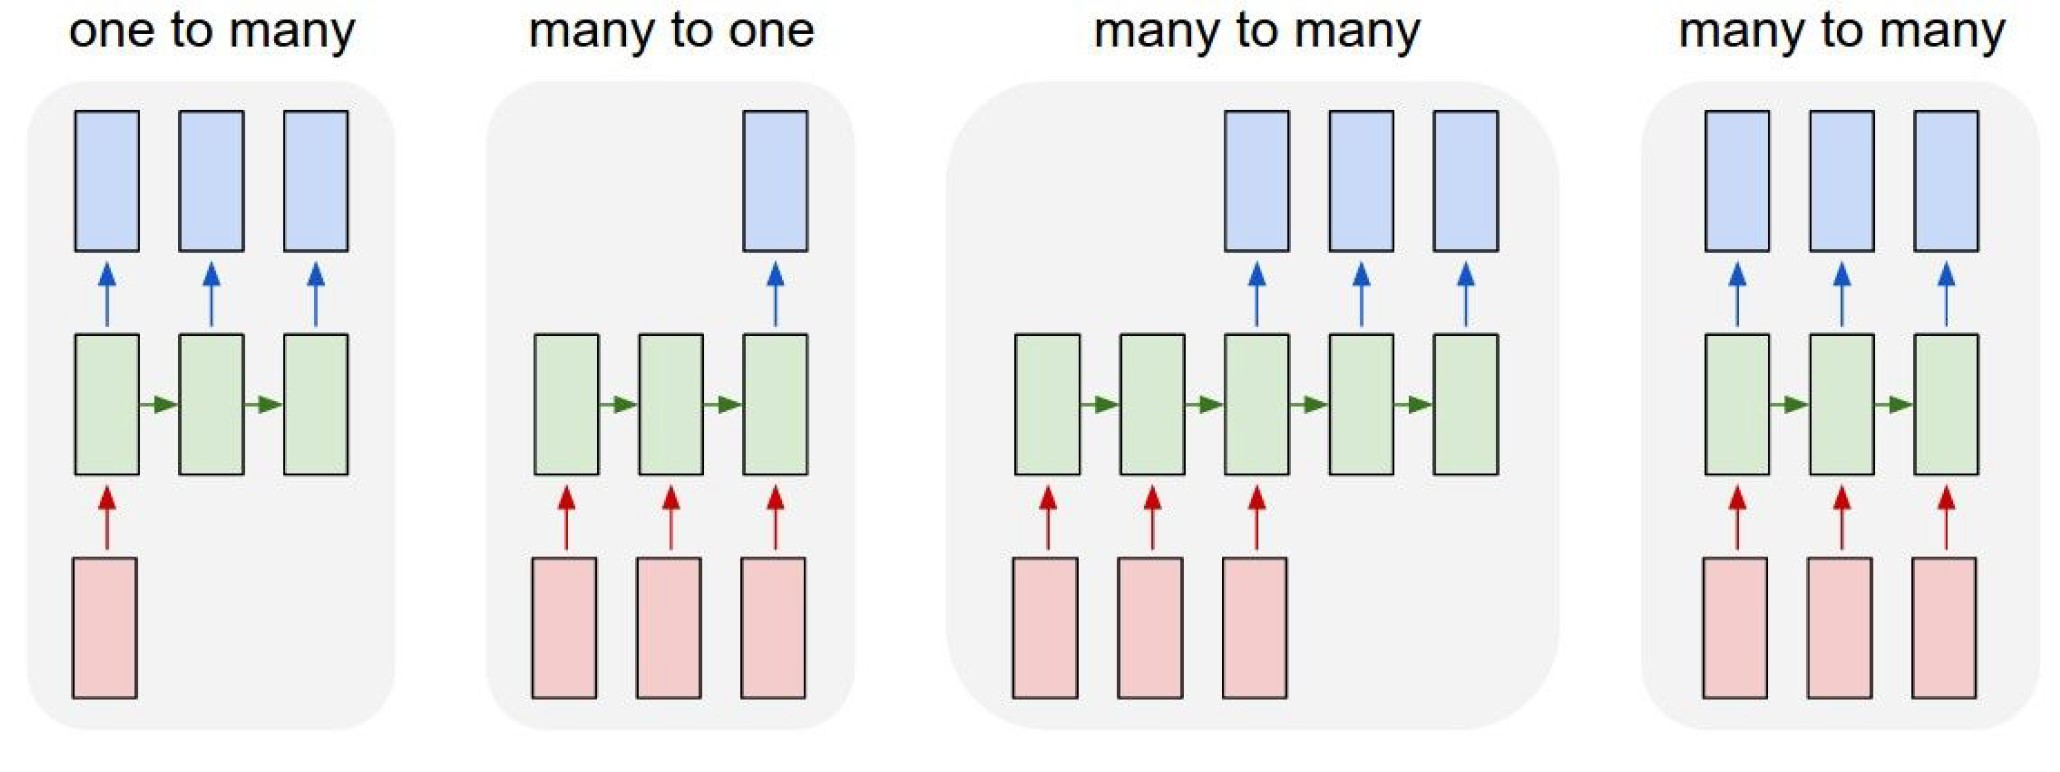
\includegraphics[width=0.8\linewidth]{images/RNN} 

}

\caption{Process sequences of different applicances of RNN.}\label{fig:RNN}
\end{figure}

Figure \ref{fig:RNN} shows different process sequences of the RNN, which
vary depending on the field of application. The red rectangles at the
bottom represent the number of inputs. Similarly, the blue rectangles
represent the outputs that come out of the RNN. The term `many' refers
to \(>1\) and is illustrated with three rectangles in the figure. The
green ones represent the hidden states \(h_i\) of all time steps and
thus can be seen as the memory of the neural network. The green arrows
show that the previous hidden state is used as input for the current
step. Starting from the left: one-to-many can be used for image
captioning (extracting sequence of words from images), many-to-one for
sentiment classification from sequence of words, many-to-many for
machine translation (sequence of words in one language to sequence of
words in another language) and many-to-many for video classification on
frame level {[}9{]}. For the prediction of the BTC/USD exchange rate in
this paper, we deal with the process many-to-one. This method combines
information from inputs and hidden states into one single prediction
value.

\begin{figure}

{\centering 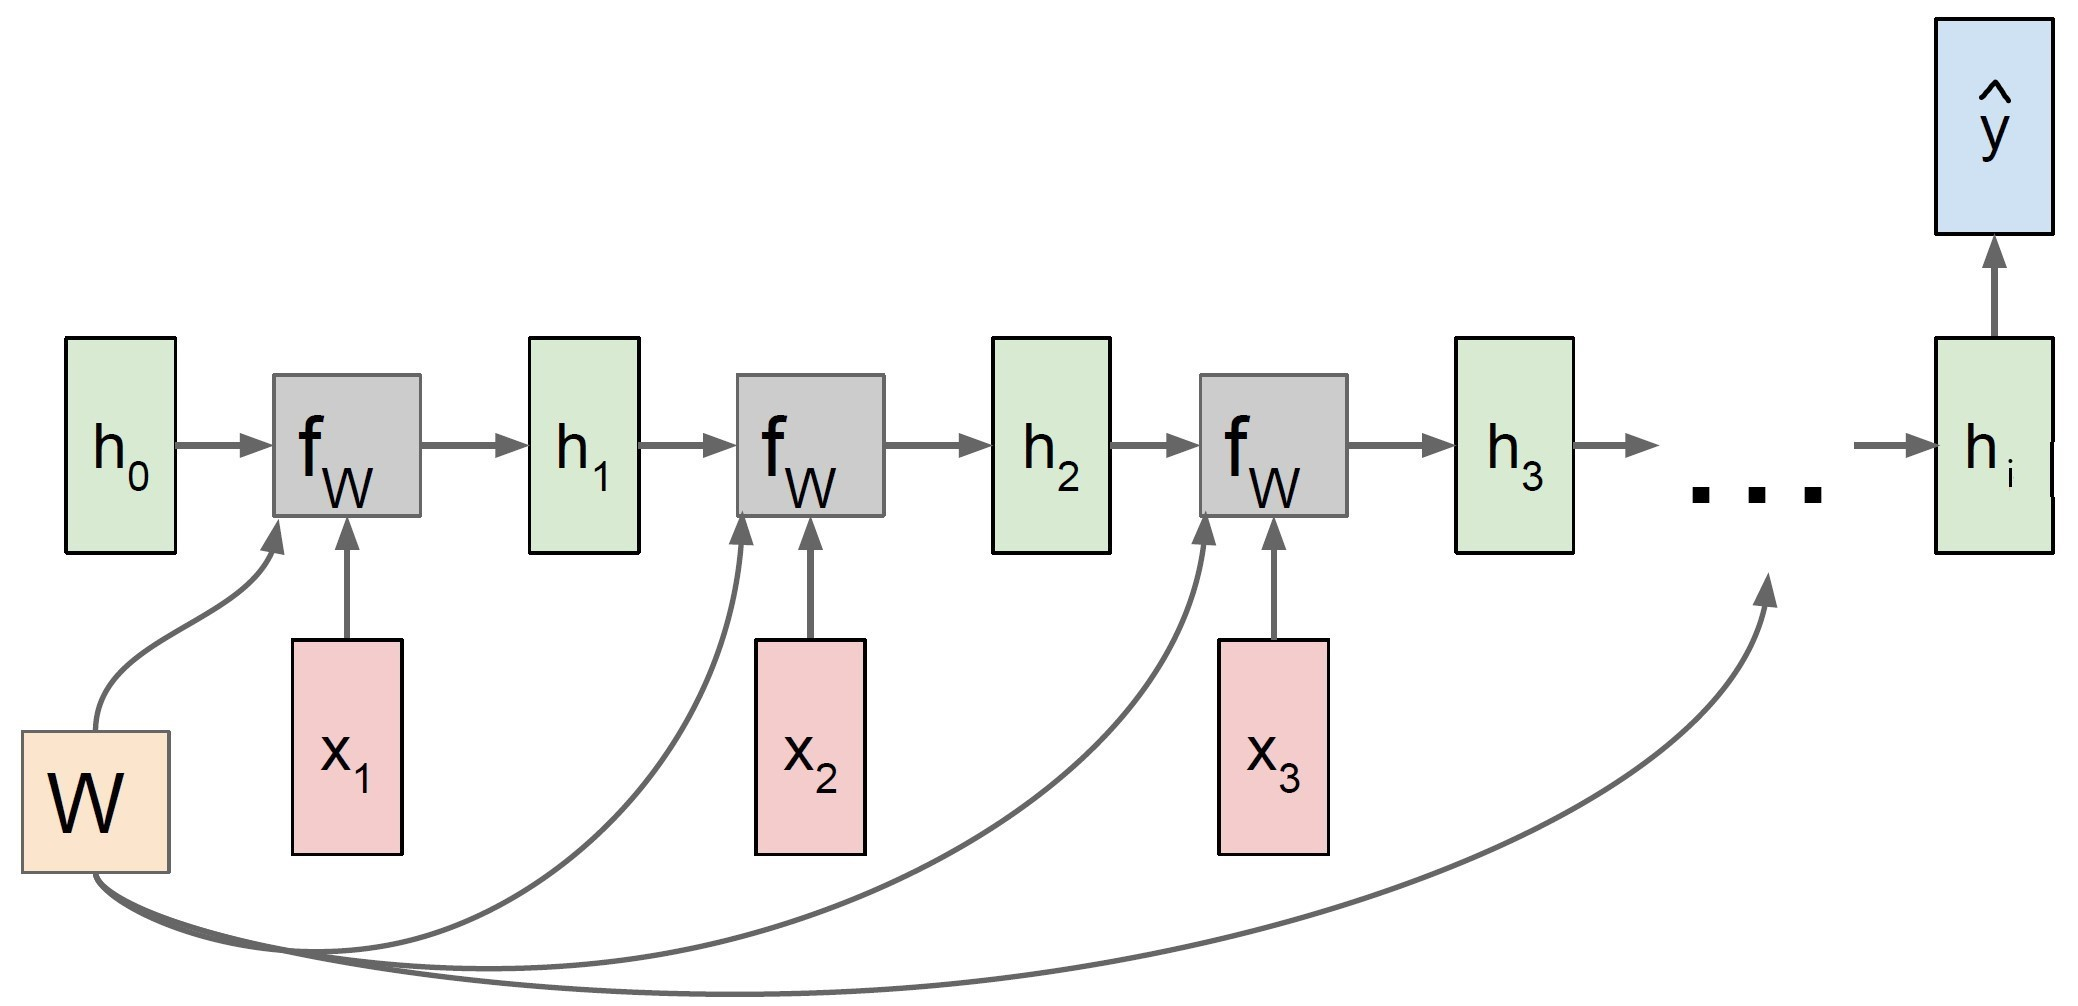
\includegraphics[width=0.7\linewidth]{images/RNN_many_to_one} 

}

\caption{Computational graph of a many-to-one RNN.}\label{fig:RNN_many_to_one}
\end{figure}

\begin{align} \label{eq:RNN_many_to_one_1}
  h_{i} & = f_{W}(h_{i-1}, x_{i}) \\
  & = \tanh(W_{h}h_{i-1} + W_{x}x_{i} + b) \nonumber 
\end{align}

Equation \ref{eq:RNN_many_to_one_1} shows how the hidden states
\(h_{i}\) are calculated at each time step, \(i\) where \(f_{W}\) is an
activation function (here: hyperbolic tangent function), \(h_{i-1}\) is
the previous state and \(x_i\) is the input vector at time step i. In
some cases, a bias term \(b\) is added to the parameters. \(W_{h}\)
represents the weight matrix for \(h_{i}\) with dimension
(length(\(h\))\(\times\)length(\(h\))). Thus, \(W_{x}\) is the weight
matrix for \(x_{i}\) with dimension
(length(\(h\))\(\times\)length(\(x\))).

\begin{align} \label{eq:RNN_many_to_one_2}
  \hat{y_{i}} = W_{y}h_{i}
\end{align}

Looking at equation \ref{eq:RNN_many_to_one_2}, \(y_{i}\) equals the
output and desired prediction of the RNN. The prediction results from
the matrix-vector product of the weight matrix \(W_{y}\) with dimension
(length(\(h\))\(\times\)length(\(y\))) and the hidden states vector
\(h\).

\hypertarget{LSTM}{%
\paragraph{2.1.5. Long-short term memory (LSTM)}\label{LSTM}}

~

\hypertarget{challenges}{%
\paragraph{2.1.6. Challenges}\label{challenges}}

~

\hypertarget{overfitting}{%
\subparagraph{2.1.6.1 Overfitting}\label{overfitting}}

~

We have encountered several challenges that can occur when using neural
networks. One of these possible problems is called overfitting. The goal
of a neural network is to build a statistical model of the training set
that is capable of generating the data. In overfitting on the other
hand, the exact conditions of the training data including noise are
reproduced. The focus is no longer on the underlying function. Last but
not least, an unnecessarily large number of parameters or epochs can be
`consumed' for this, which makes the whole process relatively
inefficient {[}8{]}.

=\textgreater{} still needs clarification how we solve these challenges
in this thesis!

\hypertarget{vanishing_gradient}{%
\subparagraph{2.1.6.2. Vanishing gradient
problem}\label{vanishing_gradient}}

~

Another characteristic that requires our attention is the vanishing
gradient problem. As explained in chapter
\protect\hyperlink{backpropagation_algorithm}{2.1.2.}, the weights of
the neural network are adjusted using the gradient of the loss function.
Thereby, the problem can occur that the gradient almost vanishes. The
error function's gradients become so small that the backpropagation
algorithm takes smaller steps towards the loss function's minima and
eventually stops learning. For example, if the derivative of an
activation function such as the logistic sigmoid function approaches
zero for extremely large or small values for \(x\). To avoid these
extreme values for \(x\), the inputs are scaled and normalized in this
paper. This ensures that the definition range is within the range where
the gradient is still large enough for the backpropagation algorithm.

=\textgreater{} still needs clarification how we solve these challenges
in this thesis!

\hypertarget{model_comparison}{%
\subsubsection{2.2. Model comparison}\label{model_comparison}}

~

This thesis sets the goal to compare the different neural networks
presented. Besides the types of neural networks, the network
architecture (number of layers and nodes) is explored. In addition, a
comparison is made with the winner of the Forecasting Competition M4,
which combines a standard exponential smoothing model with an LSTM
network. To make the comparison meaningful enough, the following two
figures are compared.

\hypertarget{sharpe_ratio}{%
\paragraph{2.2.1. Sharpe ratio}\label{sharpe_ratio}}

~

The first number refers to the performance of the trading strategy based
on the sign of the prediction \(t+1\) and is called Sharpe Ratio. Sharpe
ratio is a very powerful and widely used ratio to measure performance
and it describes return per risk.

\begin{align} \label{eq:Sharpe}
  SharpeRatio = \frac{R_{p}-R_{f}}{\sigma}
\end{align}

\(R_{p}\) represents the return of the portfolio, while \(R_{f}\) equals
the risk free rate. \(\sigma\) is the standard deviation of the
portfolios excess return (risk). For the comparison of different series,
the Sharpe Ratio needs to be annualized with \(\sqrt{365}\) as the
crypto market is open 24/7.

\hypertarget{diebold_mariano}{%
\paragraph{2.2.2. Diebold Mariano}\label{diebold_mariano}}

~

The second method used is the Diebold Mariano test, which compares the
predictive accuracy between two forecasts. First, the loss differential
\(d_{i}\) between two forecasts is defined in equation
\ref{eq:DM_loss_diff} where a loss function L of one model is subtracted
from another model. The proposed loss functions include absolute errors
(AE) and squared errors (SE) {[}10{]}. Given an expected value of
\(d = 0\), both forecasts are assumed to have the same accuracy. If the
expected value differs from zero, the null hypothesis can be rejected.
This would mean that the two methods have different levels of accuracy.

\begin{align} \label{eq:DM_hypothesis}
  H_{0}: E(d_{i}) = 0 \\
  H_{1}: E(d_{i}) \neq 0 \nonumber
\end{align}

with

\begin{align} \label{eq:DM_loss_diff}
  d_{i} = L(e_{1i}) - L(e_{2i})
\end{align}

and

\begin{align} \label{eq:DM_error}
  e_{ti} = \hat{y_{ti}} - y_{i} \\
  \text{for } t={1,2} \nonumber
\end{align}

Under the null hypothesis \(H_{0}\), the Diebold Mariano test uses the
statistics shown in equation \ref{eq:DM} and is asymptotically N(0,1)
distributed. On the other hand, the null hypothesis is rejected if the
calculated absolute Diebold Mariano value is outside \(-z_{\alpha/2}\)
and \(z_{\alpha/2}\). Thus, \(|DM|>z_{\alpha/2}\) is valid when there is
a significant difference between the predictions where \(z_{\alpha/2}\)
is the positive bound of the z-value to the level \(\alpha\).

\begin{align} \label{eq:DM}
  DM = \frac{\bar{d}}{\sqrt{\frac{2*\pi*\hat{f_{d}(0)}}{T}}} \rightarrow N(0,1)
\end{align}

where \(\bar{d}\) is the sample mean of the loss differential and
\(f_{d}(0)\) is the spectral density of the loss differential at lag k
{[}11{]}.

\begin{align} \label{eq:DM_definitions}
  \bar{d} = \sum_{i = 1}^{T}d_{i} \\
  f_{d}(0) = \frac{1}{2\pi}(\sum_{k=-\infty}^{\infty} \gamma_{d}(k))
\end{align}

In conclusion, the Diebold Mariano test helps us to understand whether
the predictions of one model turned out better by chance or due to
statistical significance.

\newpage

\hypertarget{MSE}{%
\paragraph{2.2.3. Mean Squared Error}\label{MSE}}

~

The third performance measurement method is also widely used and called
Mean Squared Error. Its calculation is very simple, for every timestep
the estimated value is subtracted from the real empirical value, squared
and then summarized and divided by the absolute number of observations
as seen in equation \ref{eq:MSE}.

\begin{align} \label{eq:MSE}
  MSE = \frac{1}{N}\sum_{i = 1}^{N}(realvalue_{i}-\hat{prediciton}_{i})^2
\end{align}  

Altough its wide application in many different sectors, the MSE has a
problem with outliers, due to the squared term, a huge outlier could
influence the MSE very strongly. Therefore one should always check for
outliers.

\newpage

\hypertarget{bitcoin}{%
\subsubsection{2.3. Bitcoin}\label{bitcoin}}

In this section bitcoin as a crypto-curreny is introduced. The
historical data is analyzed and commented. Further the technology in and
around crypto-currencies is briefly explained. A detailed explanation
would require a paper itself, therefore the explanation is done as
simple as possible.

In the following work bitcoin as a cryptocurreny is mentionend in its
short term BTC, by the meaning of US Dollars per Bitcoin.

\hypertarget{historical-analysis}{%
\paragraph{2.3.1. Historical analysis}\label{historical-analysis}}

~

The story of bitcoin began with a paper published by the name of Satoshi
Nakamoto {[}12{]}. The publisher of the document cannot be assigned to a
real person, therefore the technology inventor remains mysteriosly
unknown until today. In 2009 the first bitcoin transaction was executed.
On account of the opensource technology of bitcoin, lots of alternative
currencies were created.

Until 2013 the cryptocurrencies operated under the radar of most
regulatory institutions. Because of the anonymity of the transactions,
criminals were attracted by the newborn payment method. Headlines, such
as the seizure of 26,000 bitcoins by closing the ``Dark-Web'' Website
Silkroad through the Drug Enforcement Agency, followed moreoften in the
newspapers.

Nevertheless in 2014 more companys, such as: Zynga, D LasVegas Casinos,
Golden Gate Hotel \& Casino, TigerDirect, Overstock.com, Newegg, Dell,
and even Microsoft {[}13{]}, began to accept bitcoin as a payment
method. In 2014 the first derivative with bitcoin as an underlying was
approved by the U.S.Commodity Futures Trading Commission. 2015 an
estimated 160000 merchants used bitcoin to trade. It is observed that
the value of bitcoin is very volatile, we will discuss this in a FURTHER
XYXY section.

Let us first look a the price in Figure \ref{fig:price_btc} and the
log(price) in Figure \ref{fig:logprice_btc} and get a sense of the
chart. Note: The data in the charts start in 2014 where it was listed in
coinmarket, events between 2009 and 2014 are described without
visualization.

Around 2010 bitcoin had the first increase in price as it jumped a 100\%
from 0.0008 USD to 0.08 Dollar {[}14{]}. In 2011 the price rose from 1
USD to 32 USD within 3 months and recessd shortly after to 2 USD this
can be referred as a first price bubble in bitcoin, for the next year
the price climbed to 13 Dollars and reached a never seen level of 220
USD, only to plunge to 70 USD within a half month in April 2013. By the
end of the year a rally brought btc up to a peak of 1156 USD. The
following year brought bad news and the price slowly decreased to 315
USD in 2015 after an observed drop of 20\% after news from the trial of
Ross Ulbricht, founder of Silk road marked in Letter \textbf{A}.

From this point in time, things began to change, more volume was flushed
in the market and the price of BTC began to ascend and the real rally
began ,the BTC rose up to 20k USD / BTC on 17th September 2017
\textbf{B}. After the rise comes the fall and BTC lost value for more
than a year until \textbf{C} 2018-12-15 the trend reverted and found its
peak after 6 months in \textbf{D} 2019-06-26, but oncemore it was not
lasting for long as bitcoin lost \textbf{D} 2020-03-12 nearly half its
value in 4 days. But the story wasn't over by now, after the drop the
price of the cryptocurrency regained value, passed previous levels and
shortly after exploded, after companies like tesla and signal bought a
big chunk of bitcoins, into a maximum of 58000 USD per bitcoin.

\newpage

\begin{figure}

{\centering 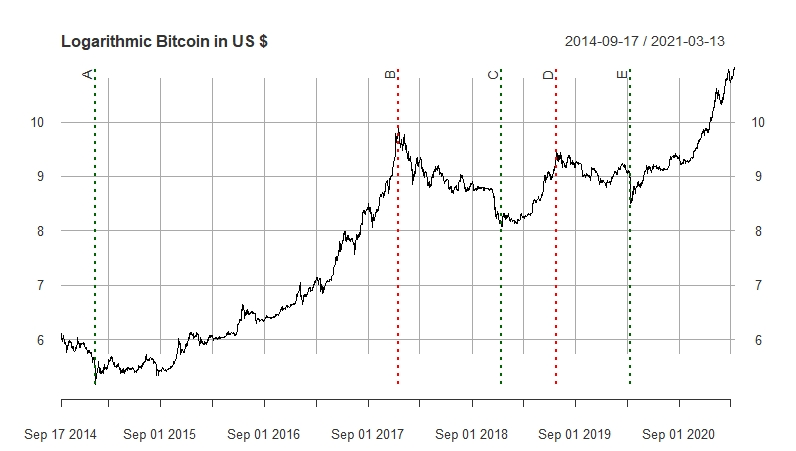
\includegraphics[width=0.8\linewidth]{images/logbtc_usd} 

}

\caption{Schematic diagram of a perceptron.}\label{fig:logprice_btc}
\end{figure}

\begin{figure}

{\centering 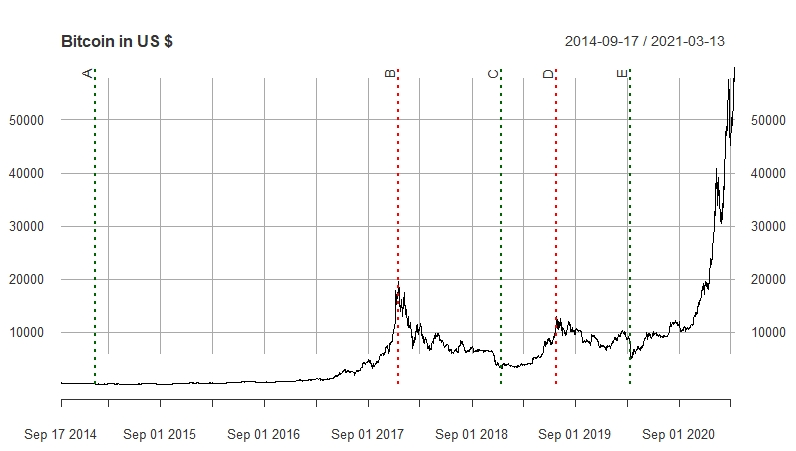
\includegraphics[width=0.8\linewidth]{images/btc_usd} 

}

\caption{Schematic diagram of a perceptron.}\label{fig:price_btc}
\end{figure}

\newpage

\hypertarget{technology-overview-sha256-hash}{%
\paragraph{2.3.2. Technology overview SHA256
Hash}\label{technology-overview-sha256-hash}}

~

\begin{itemize}
\tightlist
\item
  Block
\item
  Blockchain
\item
  Distributed Blockchain
\item
  Token
\item
  Coinbase Transaction
\item
  Public/Private Key -\textgreater{} Signing
\item
  Signature (sign, verify)
\item
  Transaction
\end{itemize}

\newpage

\hypertarget{methodology}{%
\subsection{3. Methodology}\label{methodology}}

The focus of this thesis is to predict historical prices of bitcoin
using the models listed in Chapter XX. The predictive accuracy of these
obtained predictions are compared using loss functions (Annualized
Sharpe, Diebold Mariano Test, MAE, MSE, RMSE, Mincer-Zarnowitz
Regressions). Then, based on the best models with the most accurate
predictions, trading strategies are worked out to compare with a
buy-and-hold strategy. Finally, we would like to venture into the topic
of explainability and attempt to explain why the chosen models lead to
these outcomes. The procedure of this quantitative study is described in
this chapter.

\begin{itemize}
\tightlist
\item
  Data and Analysis of Bitcoin (BTC/USD)
\item
  Defining the train and test samples (including description about calm
  and volatile phases).
\item
  Calculate predictions with the defined models (AR, NN, RNN, LSTM,
  Emponential Smoothing + NN (Slavek Smyl)).
\item
  Compare Predictions / performance with Realized Data (Annualized
  Sharpe, Diebold Mariano Test, MAE, MSE, RMSE, Mincer-Zarnowitz
  Regressions)
\item
  Explain trading strategies
\item
  Explainability for the best models
\item
  (Backup: Which models work well in which market phases?)
\end{itemize}

\hypertarget{data-and-analysis-of-bitcoin}{%
\subsubsection{3.1. Data and analysis of
Bitcoin}\label{data-and-analysis-of-bitcoin}}

The data in this paper is accessed via yahoofinance provided by
coinmarket \url{https://coinmarketcap.com/}. We use the daily ``closing
price'' of bitcoin in US Dollars with the ticker BTC-USD. Cryptoassets
are tradeble 24 hours a day 256 days a year, there is no real ``closing
price'' for the bitcoin, therefore the ``closing-Price'' is just the
last price of the day evaluated at last timestamp with timeformat UTC.

In chapter \protect\hyperlink{bitcoin}{2.3.} the bitcoin price is
visualized. For processing and analyzing the data in order to fullfill
the weak stationarity assumptions we transform the data into logreturns.

\[\mathrm{LogReturn} = \mathrm{log}(x_{t})-\mathrm{log}(x_{t-1})\]

\begin{center}\includegraphics[width=0.7\linewidth]{00_main_files/figure-latex/unnamed-chunk-11-1} \end{center}

By computing the autocorrelation oft the log\_returns, there is still
dependence visible in lag 6 and 10. This indicates dependency in
volatility-cluster, to cancel out the effect an ARMA-GARCH model is
fitted to the data and the residuals are standardized by the model
standard-deviation.

\begin{center}\includegraphics[width=0.7\linewidth]{00_main_files/figure-latex/unnamed-chunk-12-1} \end{center}

\hypertarget{comparison-of-network-architecture}{%
\subsubsection{3.2. Comparison of network
architecture}\label{comparison-of-network-architecture}}

As mentioned in chapter \protect\hyperlink{MLP}{2.1.3.}, choosing an
appropriate network architecture for bitcoin price prediction is a
crucial step in order to achieve useful forecasts while avoiding
overfitting. Due to the complexity as well as the non-linearity of
neural networks, the interpretation cannot be performed intuitively. For
this reason, an approach is pursued in which neural networks with
different numbers of layers and neurons are compared with each other by
using the MSE loss. This allows us to compare accuracy and possibly see
a connection with network architecture. The first plot in figure xy
compares different neural networks with one layer. Networks with a
maximum of six neurons are compared. These different configurations can
be seen on the x-axis. The y-axis shows the MSE values obtained with the
respective optimized model. We use ten different optimizations of each
configuration to get a better idea of a potentially systematic
relationship with the MSE. In the plot, each of the configurations is
drawn using a different color.

\begin{itemize}
\tightlist
\item
  NN for bitcoin prediction
\item
  Non-linear task
\item
  How decide the number of layers and nodes
\item
  Keep in mind rule of thumb
\item
  Test all possible configurations (with realizations = 10) and compare
  the MSE
\end{itemize}

\hypertarget{defining-train-and-test-samples}{%
\subsubsection{3.2. Defining train and test
samples}\label{defining-train-and-test-samples}}

\begin{itemize}
\item
  Describe different phases
\item
  Explain why we set train and test sample like this
\item
  Describe stable and volatile phases and why we should keep that in
  mind for predictions
\end{itemize}

\hypertarget{xy.-benchmark}{%
\paragraph{3.2.xy. Benchmark}\label{xy.-benchmark}}

To compare the models we choose two simple benchmarks the well known buy
and hold and an Ar(1) process as you can see in Figure xy and Figure
xxy.

\hypertarget{xy-evaluating-architecture}{%
\paragraph{3.3.xy Evaluating
architecture}\label{xy-evaluating-architecture}}

In order to find an appropriate model to evaluate our neural net
architecture we needed to compare different architectures of the
network. Therefore we wrote a function which compares all possible
combinations of neurons and layers for a given maximum.

For an easier understanding here is an example:

We want to know all combinations of nets for a maximum of 2 layers with
maximum 2 neurons each. With formula \ref{eq:complexity} we can compute
the number of combinations. In the example case it equals 6 nets, which
are plotted in figure \ref{figure:examples_for_function}, the input
layer is cutted down to two layers for illustration.

\begin{align} \label{eq:complexity}
\net combinations=\sum_{i=1}^{L}N^{i})
\end{align}

with:

\$L = maximum of layers \in \N \$ \$N = maximum of Neurons \in \N \$

\begin{figure}

{\centering 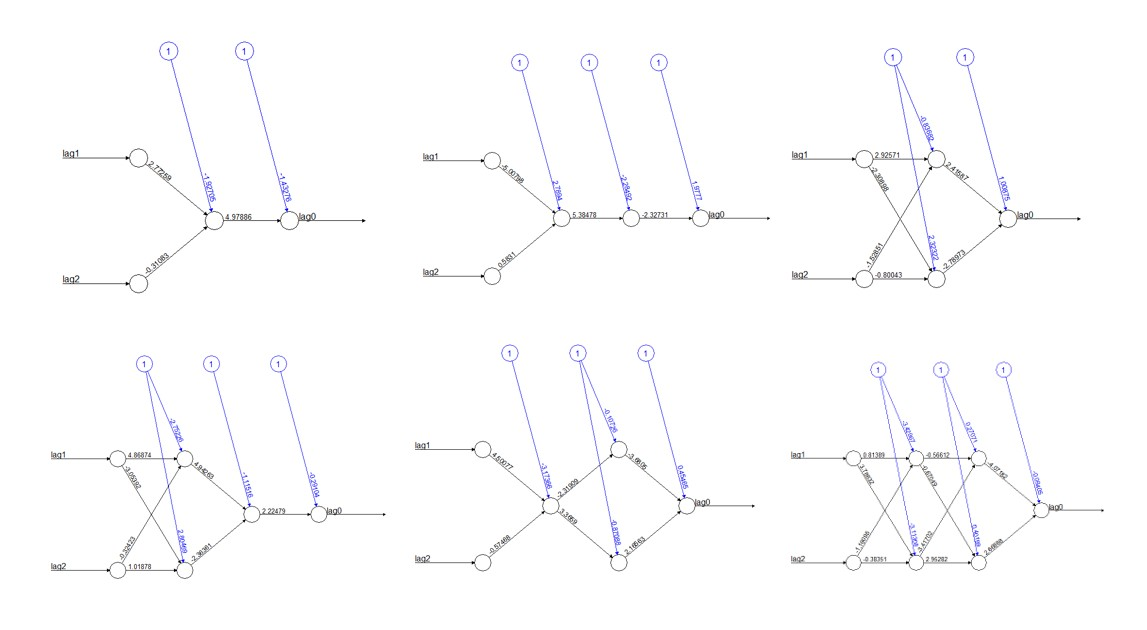
\includegraphics[width=1\linewidth]{images/examples for function} 

}

\caption{Schematic diagram of a perceptron.}\label{fig:examples_for_function}
\end{figure}

The Insample and out of sample MSE are computed and compared. Due to the
"randomness of the networks with specific numbers of layers and neurons,
multiple realisations for every single network are computed to find a
systematic deviation.

Regarding real life application of the model we evaluate performance
over different insample - out of sample

results:

\begin{itemize}
\tightlist
\item
  no need for more complexity, smaller architecture also does the job
\end{itemize}

\hypertarget{trading-strategiesg}{%
\subsubsection{3.4. Trading strategiesg}\label{trading-strategiesg}}

\begin{itemize}
\item
  Define trading strategies
\item
  Sign-trading (daily)
\item
  Vola-gewichtet trading
\item
  Define realistic fee structure for trading (Coinbase Pro, Binance,
  Kraken etc.)
\end{itemize}

\hypertarget{other-cryptocurrency}{%
\subsubsection{3.4.1. Other cryptocurrency}\label{other-cryptocurrency}}

\begin{itemize}
\tightlist
\item
  Test our best model with another time series
\end{itemize}

\hypertarget{explainability}{%
\subsubsection{3.5. Explainability}\label{explainability}}

\begin{itemize}
\item
  Performing the predictions with the two (?) best models
\item
  Include variations to find possible starting points for explainability
  (number of nodes, layers)
\end{itemize}

\hypertarget{relationship-between-accuracy-and-market-phase}{%
\subsubsection{3.6. (Relationship between accuracy and market
phase)}\label{relationship-between-accuracy-and-market-phase}}

\begin{itemize}
\tightlist
\item
  Test
\end{itemize}

\newpage

\hypertarget{results}{%
\subsection{4. Results}\label{results}}

\hypertarget{results-chapterino}{%
\subsubsection{4.1. Results chapterino}\label{results-chapterino}}

\newpage

\hypertarget{conclusion}{%
\subsection{5. Conclusion}\label{conclusion}}

Best Trading Algorithm ever!

\hypertarget{get-rich-or-die-tryin}{%
\subsubsection{5.1. Get rich or die tryin}\label{get-rich-or-die-tryin}}

Neque volutpat ac tincidunt vitae semper quis. At elementum eu facilisis
sed odio morbi quis commodo odio. Eget dolor

\hypertarget{be-gme-stock-or-not-to-be-gme-stock}{%
\subsubsection{5.2. Be GME stock, or not to be GME
stock}\label{be-gme-stock-or-not-to-be-gme-stock}}

Tellus at urna condimentum mattis pellentesque id nibh. Morbi tempus
iaculis urna id volutpat lacus laoreet. Sem fringilla

\newpage

\hypertarget{references}{%
\subsection{References}\label{references}}

\hypertarget{refs}{}
\begin{cslreferences}
\leavevmode\hypertarget{ref-perceptron_paper}{}%
{[}1{]} F. Rosenblatt, \emph{The perceptron: A probabilistic model for
information storage and organization in the brain}. Psychological
Review, 1958, pp. 386--408.

\leavevmode\hypertarget{ref-nn_learning_theoretical_foundations}{}%
{[}2{]} P. L. B. Martin Anthony, \emph{Neural network learning:
Theoretical foundations}. Cambridge University Press, 1999.

\leavevmode\hypertarget{ref-backpropagation}{}%
{[}3{]} R. Rojas, \emph{The backpropagation algorithm}. Springer Berlin
Heidelberg, 1996, pp. 149--182.

\leavevmode\hypertarget{ref-efficient_backprop}{}%
{[}4{]} G. B. O. Yann Lecun Leon Bottou, \emph{Efficient backprop}.
Image Processing Research Department AT\& T Labs, 1998, pp. 1--44.

\leavevmode\hypertarget{ref-backpropagation_proofs}{}%
{[}5{]} L. Hunsberger, ``Back propagation algorithm with proofs.''
\url{https://www.cs.vassar.edu/~hunsberg/cs365/handouts-etc/backprop.pdf}
(accessed Mar. 21, 2021).

\leavevmode\hypertarget{ref-mlp_architecture}{}%
{[}6{]} M. A. J. I. Hassan Ramchoun Youssef Ghanou, \emph{Multilayer
perceptron: Architecture optimization and training}. International
Journal of Interactive Multimedia; Artificial Intelligence, 2016, p. 26.

\leavevmode\hypertarget{ref-recipe_training}{}%
{[}7{]} A. Karpathy, ``A recipe for training neural networks.''
\url{https://karpathy.github.io/2019/04/25/recipe/} (accessed Mar. 24,
2021).

\leavevmode\hypertarget{ref-RNN}{}%
{[}8{]} M. N. S. S. Ke-Lin Du, \emph{Recurrent neural networks}.
Springer London, 2014, pp. 337--353.

\leavevmode\hypertarget{ref-RNN_Stanford}{}%
{[}9{]} S. Y. Fei-Fei Li Justin Johnson, \emph{Lecture 10: Recurrent
neural networks}. Stanford University, 2017.

\leavevmode\hypertarget{ref-DM_paper}{}%
{[}10{]} R. S. M. Francis X. Diebold, \emph{Comparing predictive
accuracy}. University of Pennsylvania, 1995.

\leavevmode\hypertarget{ref-DM_lecture}{}%
{[}11{]} U. Triacca, \emph{Comparing predictive accuracy of two
forecasts: The diebold-mariano test}. Universita dell Aquila.

\leavevmode\hypertarget{ref-bitcoin}{}%
{[}12{]} S. Nakamoto, \emph{Bitcoin: A peer-to-peer electronic cash
system}. online: www.bitcoin.org, 2008, p. 9.

\leavevmode\hypertarget{ref-A_History_of_Bitcoin}{}%
{[}13{]} U. W. Chohan, \emph{A history of bitcoin}. University of New
South Wales, Canberra, 2017.

\leavevmode\hypertarget{ref-Bitcoin_history}{}%
{[}14{]} J. Edwards, ``Bitcoins price history.''
\url{https://www.investopedia.com/articles/forex/121815/bitcoins-price-history.asp}
(accessed Mar. 01, 2021).
\end{cslreferences}

\newpage

\hypertarget{attachment}{%
\subsection{Attachment}\label{attachment}}

This project work is created with R-4.0.2 , RStudio Version 1.4.904 and
RMarkdown in collaborative working via Git / Github

\end{document}
